\documentclass[11pt]{article}
\usepackage{isma2018}

% Enter further packages required for your manuscript below.
\usepackage{graphicx}
\usepackage{amsmath}
\usepackage{amsfonts} %potrzebne do \mathbb{S}
\usepackage{amssymb}
\newcommand{\D}{\displaystyle}
\usepackage[numbers,square,sort&compress]{natbib}

%%%%%%%%%%%%%%%%%%%%%%%%%%%%%%%%%%%%%%%%%%%%%%%%%%%%%%%%%%%%%%%%%%%
% The "hyperref" package may be used in conjunction with PDFLatex %
% to add document information to the generated PDF file. Please,  %
% fill out the same title, author(s) and keywords as on the paper %
% submission form. Note, that the "hypperref" package should be   %
% loaded as the last.                                             %
%                                                                 %
% If you are not using PDFLatex, delete or comment the following  %
% lines. In that case, the conference secretary will add the      %
% document information to your PDF file.                          %
%%%%%%%%%%%%%%%%%%%%%%%%%%%%%%%%%%%%%%%%%%%%%%%%%%%%%%%%%%%%%%%%%%%

\usepackage[pdftex]{hyperref}
\usepackage{color}

\hypersetup{a4paper = true,
	pdfpagemode = None,
	pdfstartview  = FitH,
	citebordercolor = 1 1 1,
	filebordercolor = 1 1 1,
	linkbordercolor = 1 1 1,
	urlbordercolor = 1 1 1}
\hypersetup{pdftitle  = {Manuscript preparation instructions},
	pdfauthor = {P. Kruczek},
	pdfkeywords = {ISMA2018, USD2018, template}}

\title{Multi-fault diagnosis based on bi-frequency cyclostationary maps clustering}

\author{\textbf{P. Kruczek $^1$, J. Wodecki $^2$, A. Wy{\l}oma{\'n}ska $^1$, R. Zimroz $^2$, K. Gryllias $^{3, 4}$
} \\
  $^1$ KGHM Cuprum Ltd, R \& D Centre, \\
  Sikorskiego 2-8, 53-659 Wroclaw, Poland, \\
  e-mail: \textbf{p.kruczek@cuprum.wroc.pl} 
% Uncomment this block to add multiple (different) affiliations.
 \\ [3mm]
 $^2$ Faculty of Geoengineering, Mining and Geology, Wroc{\l}aw University of Science and Technology, \\
 Na Grobli 15, 50-421 Wroclaw, Poland
 \\ [3mm]
 $^3$ KU Leuven, Department of Mechanical Engineering, \\
 Celestijnenlaan 300 B, B-3001, Leuven, Belgium 
 \\[3mm]
$^4$ Dynamics of Mechanical and Mechatronic Systems, Flanders Make, Belgium
  }

\date{}

\begin{document}

\abstract{Condition monitoring of rotating machinery is a field of intensive research. One of the most powerful diagnostic tools are based on the cyclostationary properties of the signals. In this paper an advanced signal processing diagnostic tool is introduced based on  Cyclic Spectral Coherence (CSC). The CSC is represented in a 3D bi-frequency map, which can be  integrated on the carrier frequency  leading to 2D vectors. Fault diagnosis is more challenging in the case of complex signals, which often contain many different sources of noise and more than one fault components. Therefore, a new methodology is proposed, which focuses on the separation of the information linked to different types of defects by applying tools for clustering on the  CSC map. As a result, each cluster will contain the separated information of each fault. Moreover, a CSC map will be recreated based on each cluster and the integrated maps will include only one type of defect. The methodology is tested  on real signals recorder on heavy duty machine located in an underground mine.}

\maketitle

\section{Introduction}

Modern condition monitoring techniques are able to diagnose damages at early stage, in complex machines operating under varying speed/load conditions in presence of heavy impulsive noise \cite{wylomanska2017application,borghesani2013new,schmidt2018novelty,gryllias2018application,javorskyj2016periodically}. In \cite{kruczek2017cyclic} a method for cyclic source extraction from complex vibration signals has been presented. Moreover the application of the Schur filter for local damage detection in machinery has been illustrated in \cite{makowski2014new}.
However, in order to face such challenging tasks in an industrial context, researchers continuously develop and propose new advanced signal processing techniques and diagnostic procedures \cite{wylomanska2016impulsive, hu2016development, michalak2017application}. Often the methodologies are complex for use by the machinery operators and an expert is required in order to interpret the results. This is a typical obstacle for most 3-dimensional representations of signals, such as different Time-Frequency Maps, the Bi-Spectrum and the Cyclic Spectral Coherence map\cite{kruczek2017multiple}. Obviously, the final result depends on the level of complexity of both the method and the analyzed signals. 
The real industrial signals are complex and usual contaminated by noise. Experts prefer to use methods which are easy to be interpreted. Therefore, there is a ever growing need for automatic damage detection methods \cite{wodecki2018optimal}. To overcome the abovementioned limitations, an automatic procedure is proposed in this paper in order to facilitate the understanding of such 3D maps and to provide a simple picture commonly presented in textbooks. In some sense the proposed methodology can be consider as a source separation technique in the bi-frequency domain. 

The Cyclic Spectral Coherence (CSC) is a 3D bi-frequency map, providing information about the modulation and the carrier frequencies, which are present in vibration signals. Moreover, characteristic fault frequencies related to the local damage can be observed in the CSC. Furthermore, these 3D maps can be integrated over the whole frequency band or on optimally selected bands leading to 2D vectors which are considered equivalent to the classical Squared Envelope Spectrum (SES).
However, in case of heavy duty machines with multiple faults located at different shafts (rotating at different speeds) it might happen that the fault related patterns in a CSC map integrated to a 2D envelope spectrum are hard to be identified. On the other hand by applying a clustering technique of the map, the content related to a given fault could be separated and finally instead of one figure with multiple faults, several figures with a single fault could be obtained. In this way the analysis and the interpretation of the results might be easier.

In this paper a complete procedure is proposed in order to automatically process a 3D CSC map where two faults are present at different component (i.e. fault frequencies) and different carrier frequencies. The procedure is applied on a real signal from a two stage gearbox operating in a heavy duty drive unit used in mining applications. Based on the results, source separation in a bi-frequency domain is possible after the integration of the new map in order to calculate an Envelope Spectrum (ES) \cite{randall2001relationship}. The structure of ES is much clearer and allows to easily identify the damage. The clustering algorithm used in this paper is based on the Expectation Maximization (EM) algorithm \cite{dempster1977maximum, kaufman2009finding}. 

The paper is organized as follows. The proposed methodology is first described in section \ref{sec_meth}. The CSC and the EM methods are presented and the clustering of the map is explained. Moreover in section \ref{sec:application} the application of the method to real data is presented. The paper closes with some conclusions.

\section{Methodology}\label{sec:sec_meth}
The proposed procedure is a combination of three techniques, namely the CSC representation, the clustering based on the EM algorithm and the integration of the obtained new CSC maps (for each cluster separately). In fact all these techniques are well-known, however their combination is a novel approach in condition monitoring, focusing specifically on multiple fault cases and provides promising results. In this section the definitions and the main properties of the proposed methodology are briefly introduced. Furthermore, their fusion is illustrated and described. 

\subsection{Cyclic Spectral Coherence}
The Cyclic Spectral Coherence is a function, which depends on the modulation and the carrier frequency. It has been introduced by Antoni in 2007~\cite{antoni2007cyclic} and it has been proven as a powerful tool to indicate the cyclostationary property of signals.  The Cyclic Power Spectrum (CPS) $S_X(f;\alpha)$ of a signal $\mathbf{x}$ can be estimated based on the equation:
\begin{equation}
\label{eq:CPS}
S_X(f;\alpha)=\lim_{L\to \infty}\D{1\over L}\mathbb{E}\left(\mathcal{F}_{\mathbf{x},L}(f+\D{\alpha \over 2})\overline{\mathcal{F}_{\mathbf{x},L}(f-\D{\alpha \over 2})}\right),
\end{equation}
where $\mathcal{F}_{\mathbf{x},L}(f)$ is the Fourier transform of the signal $\mathbf{x}$ calculated on an interval of length $L$.
CPS is used in order to measure the spectral dependency in the analyzed signal and it relies on the modulation ($\alpha$) and the carrier ($f$) frequencies. It is expected that the CPS satisfy the equation $\left|S_X(f;\alpha)\right|>0$ for a cyclostationary signal for some $\alpha\neq 0$. Furthermore, the definition of CSC can be formulated as:
 ~\cite{antoni2007cyclic}:
\begin{equation}
\label{eq:SC}
CSC(f;\alpha)=\left|\gamma_X(f;\alpha)\right|^{2}=\D { \left|S_X(f;\alpha)\right|^2 \over S_X(f+\D{\alpha \over 2};0)S_X(f-\D{\alpha \over 2};0)}.
\end{equation}
The Cyclic Spectral Coherence is a normalized CPS and thus its value is bounded in the interval $(0,1)$. It is expected that the CSC describe the spectral cyclic autocorrelation of the signal. Therefore, it can be used as a cyclostationary indicator. Once the $\left|\gamma_X(f;\alpha)\right|^{2}$ is significantly higher than 0, then the signal presents a cyclostationary property for a modulation frequency $T=1/\alpha$ and a carrier frequency $f$.

The estimation of the CSC can be performed directly using the CPS estimator. Thus the following formula is obtained:
\begin{equation}
\left|\hat{\gamma}_X(f;\alpha)\right|^{2}=\D { \left|\hat{S}_X(f;\alpha)\right|^2 \over \hat{S}_X(f+\D{\alpha \over 2};0)\hat{S}_X(f-\D{\alpha \over 2};0)},
\end{equation} 
where $\hat{S}_X(f;\alpha)$ is an estimator of the CPS.
It is worth mentioning that the CPS can be estimated based on different methods\cite{antoni2007cyclic2} but here the Welch method is used.

\subsection{Expectation - Maximization clustering algorithm}
In this section the Expectation-Maximization  method, for clustering the data, is described \cite{sundberg1974maximum,dempster1977maximum}. 
The Expectation – Maximization (EM) is an iterative optimization method for the estimation of unknown parameters for given measurement data $X$. EM is particularly useful for separating mixtures of Gaussian distributions (or any other distribution) over the considered feature space. It consists of two main steps: the Expectation (E-step) and the Maximization (M-step), which are iterated until convergence. 

Firstly, it is assumed that the following N data points are observed in a $D$-dimensional space 

$X=\{\overrightarrow{x}_1,\overrightarrow{x}_2,\dots \overrightarrow{x}_N\}$

Furthermore, $N$ points are drawn from a $D$-dimensional Gaussian distribution. The $l$-th distribution is characterized by the parameters $\theta_l=\{\overrightarrow{\mu}_l,\Sigma_l\}$, where $\overrightarrow{\mu}_l$ is the $D$-dimensional mean and $\Sigma_l$ is the covariance matrix. we  assign Then a prior probability $\alpha_l$ is assigned to the $l$-th Gaussian, where $\sum_{l=1}^N \alpha_l=1$.

% Furthermore, it is assumed that, the drawn Gaussian distribution for given element $X$ is unknown. However, it is known that each element of the dataset $X$ is characterized by the following mixture probability density function:
% \begin{equation}
%     p(\overrightarrow{x}|\Theta)=\sum_{l=1}^K \alpha_l p_l (\overrightarrow{x}|\theta_l),
% \end{equation}
% Where $\Theta$ represents all the parameters involved in the description of the mixture:
% \begin{equation}
%     \Theta=(\alpha_1,\alpha_2,\dots,\alpha_K;\theta_1,\theta_2,\dots,\theta_K).
% \end{equation}
% As it is expected, the $l$-th Gaussian in the mixture is given by:
% \begin{equation}
% \label{eq:distribution1}
%     p(\overrightarrow{x}|\theta_l)=\frac{1}{(2\pi)^{d/2}|\Sigma_l|^{1/2}}\exp{\left(-\frac{1}{2}(\overrightarrow{x}-\overrightarrow{\mu}_l)^T\Sigma_l^{-1}(\overrightarrow{x}-\overrightarrow{\mu}_l)\right)}
% \end{equation}
% If we assume that the $N$ observations in $X$ are independent, we can write the following expression for the probability distribution for all of the observations in $X$:
% \begin{equation}
% \label{eq:distribution2}
%      p(\overrightarrow{x}|\Theta)=\prod_{i=1}^Np(\overrightarrow{x}_i|\Theta)=\prod_{i=1}^N\left( \sum_{l=1}^K\alpha_lp_l(\overrightarrow{x}_i|\theta_l) \right).
% \end{equation}
% Substituting the individual Gaussians from Equation (\ref{eq:distribution1}) in (\ref{eq:distribution2}), we can write  the probability distribution for all of our dataset:
% \begin{equation}
% \label{eq:distribution3}
%     p(\overrightarrow{x}|\Theta)=\prod_{i=1}^N\left( \sum_{l=1}^K\alpha_l\frac{1}{(2\pi)^{d/2}|\Sigma_l|^{1/2}}\exp{\left(-\frac{1}{2}(\overrightarrow{x}-\overrightarrow{\mu}_l)^T\Sigma_l^{-1}(\overrightarrow{x}-\overrightarrow{\mu}_l)\right)} \right).
% \end{equation}
% If the parameter set $\theta$ is known, then $ p(\overrightarrow{x}|\Theta)$ is a probability distribution for the dataset $X$. However, the main  goal is to estimate $\Theta$ from a given set of observations $X=\{\overrightarrow{x}_1,\overrightarrow{x}_2,\dots \overrightarrow{x}_N\}$, thus it is prefered to consider the right hand side in equation (\ref{eq:distribution3}) as the likelihood that informs how likely the known observations in $X$ are for candidate values for the elements of $\Theta$. To make this fact more explicit, we rewrite equation (\ref{eq:distribution3}) as:
    
%     \begin{equation}
%         L(\Theta|X)=\prod_{i=1}^N\left( \sum_{l=1}^K\alpha_l\frac{1}{(2\pi)^{d/2}|\Sigma_l|^{1/2}}\exp{\left(-\frac{1}{2}(\overrightarrow{x}-\overrightarrow{\mu}_l)^T\Sigma_l^{-1}(\overrightarrow{x}-\overrightarrow{\mu}_l)\right)} \right)
%     \end{equation}
% Our goal is to construct a Maximum Likelihood estimate for $\Theta$ by seeking $\Theta^*$ that maximizes the log-likelihood:
% \begin{equation}
%   \Theta^*=\textrm{argmax}_{\Theta}\ln(L(\Theta|X)).
% \end{equation}
% Then 
% % \begin{align}
% %     B'_m(x)&=\sum_k \binom{m}{k}(m-k)B_kx^{m-k-1} 
% %     =\nonumber\\
% %     &=
% %     m\sum_k \binom{m-1}{k}B_k x^{m-1-k}
% %     =\nonumber\\
% %     &=
% %     mB_m-1(x)
% % \end{align}
% \begin{align}
%     \Theta^*=\textrm{argmax}_{\Theta}\ln\left[\prod_{i=1}^N\left( \sum_{l=1}^K\alpha_l\frac{1}{(2\pi)^{d/2}|\Sigma_l|^{1/2}}\exp{\left(-\frac{1}{2}(\overrightarrow{x}-\overrightarrow{\mu}_l)^T\Sigma_l^{-1}(\overrightarrow{x}-\overrightarrow{\mu}_l)\right)} \right)\right]\nonumber
%     \\
%     =\textrm{argmax}_{\Theta}\left[\sum_{i=1}^N\left(\ln \sum_{l=1}^K\alpha_l\frac{1}{(2\pi)^{d/2}|\Sigma_l|^{1/2}}\exp{\left(-\frac{1}{2}(\overrightarrow{x}-\overrightarrow{\mu}_l)^T\Sigma_l^{-1}(\overrightarrow{x}-\overrightarrow{\mu}_l)\right)} \right)\right]
%     \label{eq:MLE}
% \end{align}
% According to equation (\ref{eq:MLE}) it is a challenging task to determine  a $\Theta$ that maximizes the log-likelihood, because we are dealing with the logarithm of a summation of exponentials. In this case the usual convenience afforded by the fact that the logarithm of an isolated Gaussian distributions reduces to a simple quadratic form cannot help us here. This is why we need the EM algorithm.



In the first iteration, the algorithm has to be fed with some initial values of parameters $\Theta$. This can be done by picking random means, covariances and distribution weights, but it is a good practice to pre-estimate the means $\overrightarrow{\mu}_l$  using a simpler algorithm like the k-means or the hierarchical clustering  and then to compute the covariance matrices $\Sigma_l$ based on the results of this pre-clustering as well as the set weights $\alpha_l$ in order to normalized the amount of points in each cluster.
 \begin{itemize}
     \item E-step
 \end{itemize}
This step is responsible for the estimation of the probability that a data point $\overrightarrow{x}_i$  belongs to a cluster $\theta_l$:
\begin{equation}
    p(\theta_l|\overrightarrow{x}_i)=\alpha \frac{1}{(2\pi)^{\frac{D}{2}}|\Sigma_l|^{\frac{1}{2}}}\exp\left(-\frac{1}{2}(\overrightarrow{x}_i-\overrightarrow{\mu}_l)^T\Sigma_l^{-1}(\overrightarrow{x}_i-\overrightarrow{\mu}_l)\right).
\end{equation}
    \begin{itemize}
        \item M-step
    \end{itemize}
In this step the algorithm estimates the new parameters $\Theta$ of the probability distribution of each cluster for the next iteration. Firstly the mean for each cluster is computed by calculating the mean of all points in function of the relevance degree of each point:
\begin{equation}
    \mu_l(t+1)=\frac{\sum_{i=1}^N p(\theta_l|\overrightarrow{x}_i)\overrightarrow{x}_i}{\sum_{i=1}^N p(\theta_l|\overrightarrow{x}_i)}.
\end{equation}
Then the covariance matrices can be computed, based on the conditional probability of the cluster occurrence:
\begin{equation}
    \Sigma_l(t+1)=\frac{\sum_{i=1}^N p(\theta_l|\overrightarrow{x}_i)(\overrightarrow{x}_i-\overrightarrow{\mu}_l(t))^T(\overrightarrow{x}_i-\overrightarrow{\mu}_l(t))}{\sum_{i=1}^N p(\theta_l|\overrightarrow{x}_i)}.
\end{equation}
At the end of the M-step, the probability of occurrence of each class is computed through the mean of probabilities of each point from the cluster in function of the relevance degree:
\begin{equation}
    \alpha_l(t+1)=\frac{1}{N}\sum_{i=1}^{N}p(\theta_l|\overrightarrow{x}_i), l=1,\dots,K.
\end{equation}
It is very important to remember the limitations of the EM methodology. It only approximates the maximum likelihood estimate and do not find the theoretical value. If the likelihood function has multiple peaks (non-concavity case) EM will not necessarily find the global optimum of the likelihood. In practice, it should not been performed only once. It is very common to start EM multiple times with multiple random initial guesses and choose the one with the largest likelihood as the final estimate for $\Theta$. In this work EM has been run 10 times.
%
%
\subsection{Clustering of the map}
In this section the clustering of the bi-frequency map is described. The CSC map defined in section \ref{eq:SC} is analysed. The procedure of  map clustering is shown in Fig. \ref{fig:clustering}. 
\begin{figure}[h!]
\begin{center}
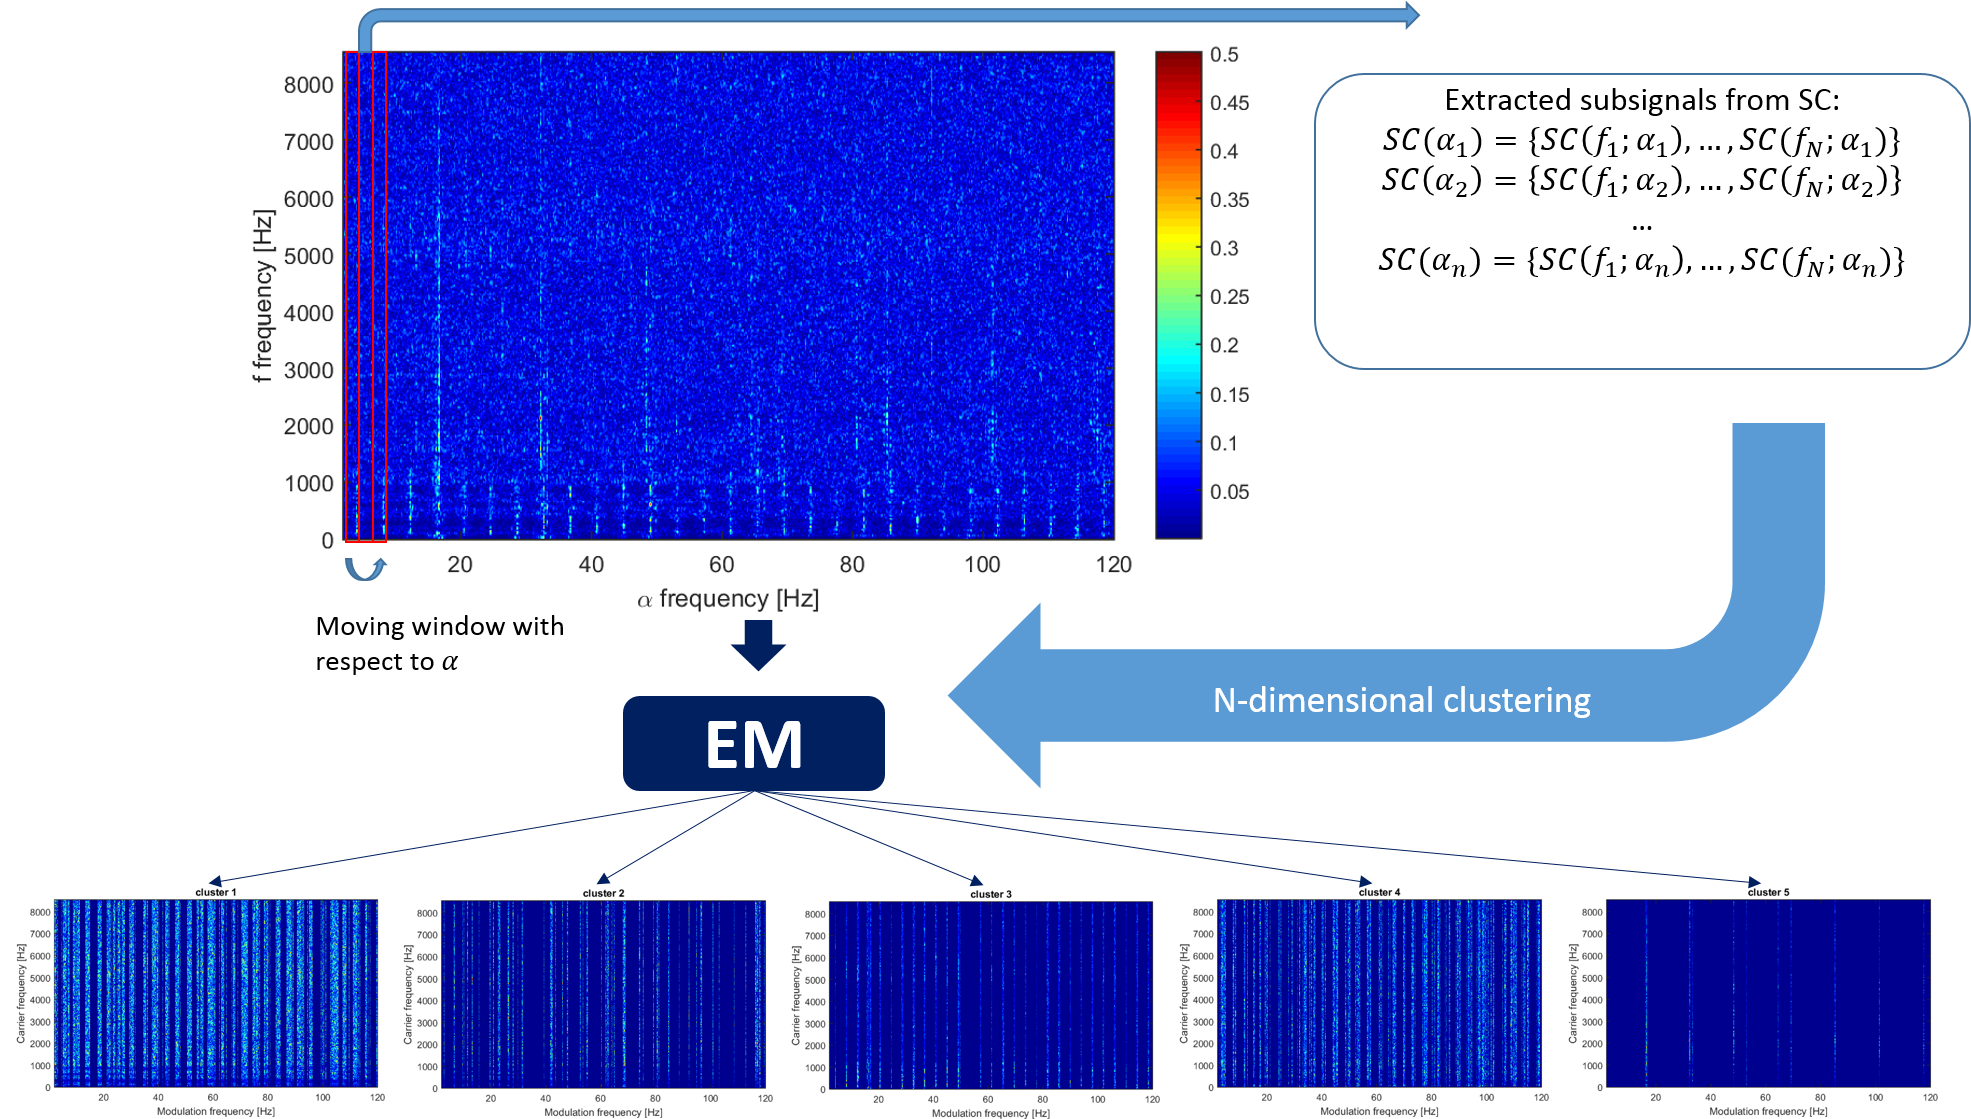
\includegraphics[width=\textwidth]{wykresy/schemat1.png}
\caption{The schema of CSC map clustering.}
\label{fig:clustering}
\end{center}
\end{figure}
In the first step, the CSC map is computed for the given signal. Therefore the two dimensional function of modulation and carrier frequencies is obtained having for example size $N \times n$.  Then, the subsignals are extracted from the map. For example, for given i-th modulation frequency $\alpha_i$ the following one dimensional function $SC(\alpha_i)=\{SC(f_1;\alpha_i),\dots ,SC(f_1;\alpha_i)\}$ is considered. These $N$ dimensional vectors are the inputs of EM. In the next step, the number of clusters should be selected. In order to determine the optimal number of clusters the Silhouette criterion can be used. Each of the subsignals  is assigned to an appropriate group using the EM. Finally, the CSC can be plotted for each cluster separately. It is expected that each cluster will contain information about only one signal component. 
%
%
\subsection{CSC map integration}
It can be observed that the CSC provides information about the excitation for given modulation and carrier frequencies. On the other hand, the total energy of a given frequency band is also interesting for diagnostic purposes. In such case,  the CSC map can be integrated with respect to the carrier frequency and the given modulation frequency \cite{randall2001relationship}. Therefore, the following formula for the integrated  CSC in the frequency band $[f_1,f_2]$ can be introduced:
\begin{align}
 ISC(\alpha;f_1,f_2)=\sum_{f=f_1}^{f_2}\left|SC(\alpha,f)\right|,
\end{align}
where $\alpha$ is a modulation frequency bin. As a result, the one dimension function of modulation frequency is obtained. The integrated map present values which are significantly higher than zero for a cyclostationary signal and are related to the the well-known envelope spectrum.

\section{Application}
\label{sec:application}
The proposed methodology is applied, tested and evaluated on a real data case. The processed signal has been captured using an accelerometer positioned on a belt conveyor's gearbox under operation. The gearbox consists of a bevel stage and a spur stage. The machine is located in an underground copper mine. The operational conditions are harsh and the signal is highly contaminated by external noise. The raw signal is presented in Fig. \ref{fig:raw_signal}. Its length is equal to 10 seconds while the sampling frequency is 17066~Hz and the rotation frequency of the first shaft is equal to 16.5 Hz.

\begin{figure}[h!]
\begin{center}
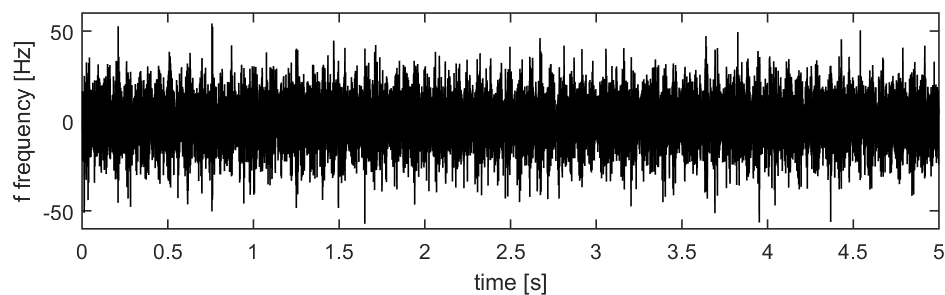
\includegraphics[width=\textwidth]{wykresy/_sygnal.png}
\caption{The raw vibration signal measured on a belt conveyor's gearbox.}
\label{fig:raw_signal}
\end{center}
\end{figure}
The machine under monitoring contains two different local gear faults, one mounted on the first shaft and one on the second one. Their fault frequencies are equal to 16.5~Hz and 4.17~Hz respectively. Following the methodology described above, it is expected that two separate clusters, one for each fault will be created. In the first step, the Cyclic Spectral Coherence map is computed (Fig. \ref{fig:SC}). Analysing carefully the map, a cyclic excitation can be observed at low carrier frequencies with a modulation frequency equal approximately to 4.1 Hz. Furthermore a wide range excitation can be identified for modulation frequencies around 16.5 Hz and its multiples. Therefore, the SC contain the information about both local damages of the analyzed machine.
%
\begin{figure}[h!]
\begin{center}
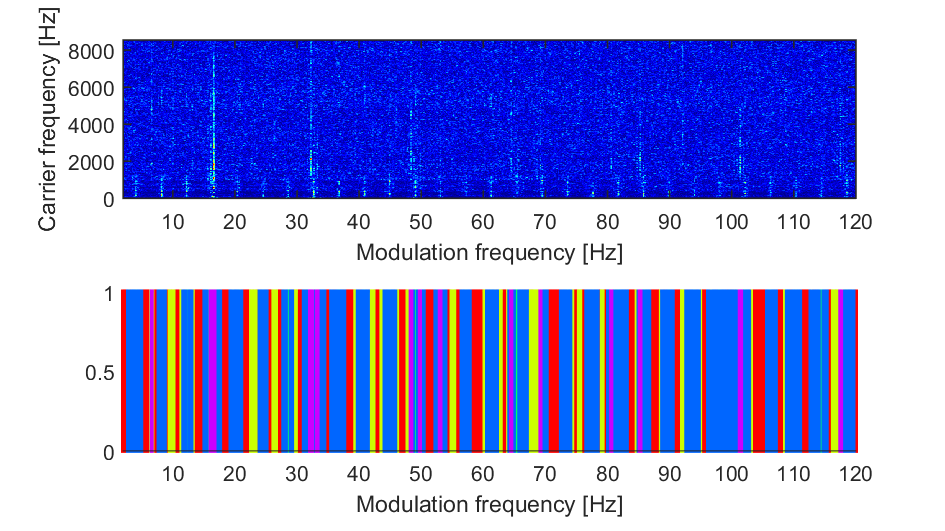
\includegraphics[width=\textwidth]{wykresy/212_SC_clusters.png}
\caption{The Cyclic Spectral Coherence map (upper panel) and the assigned clusters from EM (bottom panel).}
\label{fig:SC}
\end{center}
\end{figure}
%
In order to automatically separate the information for both damages, the SC map could be clustered using the EM method. In clustering methods, it is especially important to select a priori the appropriate number of clusters. Therefore the Silhouette criterion has been used in order to determine the cluster number which is selected equal to 5. The assigned clusters are presented in Fig. \ref{fig:SC}. Each cluster is marked with a specified color. It can be observed that each local damage has been assigned to a different cluster. The clusters contain only the components related to the local faults. In further analysis, only clusters no. 3 and no. 5 are considered as they contain information about the two local damages. Moreover the SC maps are reconstructed based on the clusters and are presented separately. The map containing the information about the damage on the second shaft (4.1~Hz) is presented in Fig. \ref{fig: SC_cluster3}. It can be noted that the energy of the reconstructed map is concentrated at a low carrier frequency band around to 1500~Hz.
%
\begin{figure}[h!]
\begin{center}
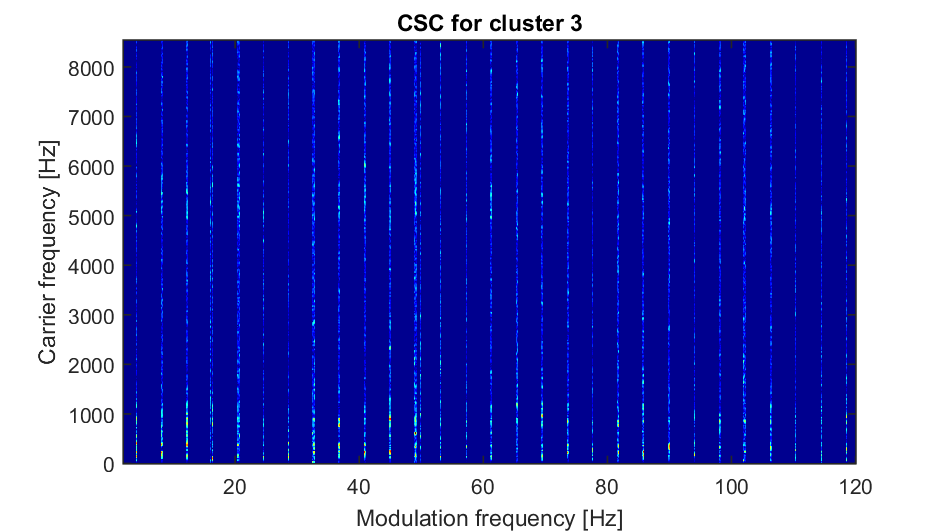
\includegraphics[width=\textwidth]{wykresy/212_SC_cluster_3.png}
\caption{The Cyclic Spectral Coherence map for the cluster containing information about the damage on the second shaft.}
\label{fig: SC_cluster3}
\end{center}
\end{figure}
%
The SC map of the cluster which contains diagnostic information for the damage related to the first shaft (16.5~Hz) is presented in Fig. \ref{fig:SC_cluster5}. In this case a wide band excitation can be identified. 
\begin{figure}[h!]
\begin{center}
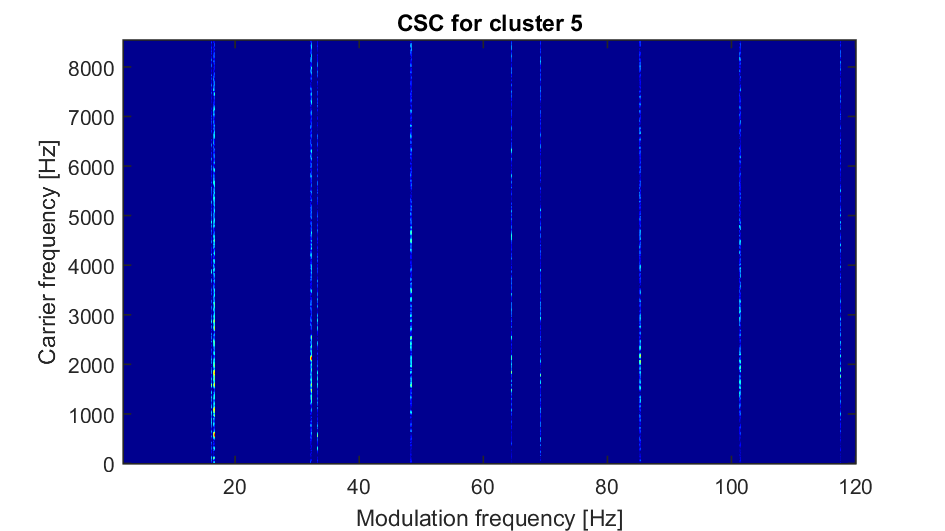
\includegraphics[width=\textwidth]{wykresy/212_SC_cluster_5.png}
\caption{The Spectral Coherence map of the cluster containing information about the damage on the first shaft.}
\label{fig:SC_cluster5}
\end{center}
\end{figure}
%
Finally the integrated maps for the clusters no 3 and no 5 are computed. In Fig. \ref{fig:intSC3} the integrated SC for the cluster containing information about the damage related to the second shaft is presented. The excitation of 4.1~Hz and its multiples are clearly observed. 
\begin{figure}[h!]
\begin{center}
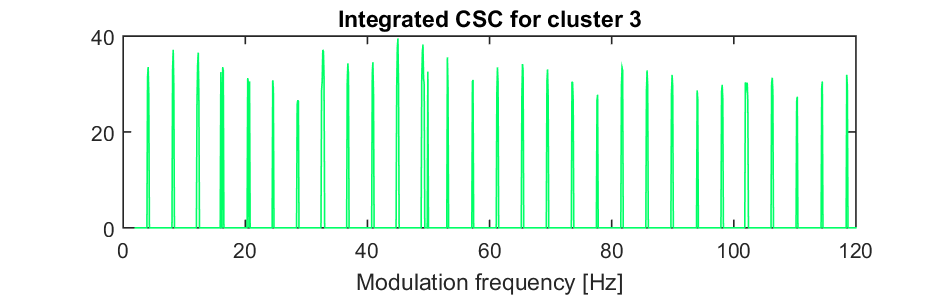
\includegraphics[width=\textwidth]{wykresy/212_cluster_sum_3.png}
\caption{The Integrated Spectral Coherence map of the cluster containing information about the damage on the second shaft.}
\label{fig:intSC3}
\end{center}
\end{figure}
In Fig. \ref{fig:intSC5} the integrated map for the cluster no 5 is presented. In this case, the map contains  information about the damage of the first shaft. The excitation of 16.5~Hz and its multiples can be clearly identified. Therefore, only the signal component related to the local damage of the gear mounted on the first shaft is present.
\begin{figure}[h!]
\begin{center}
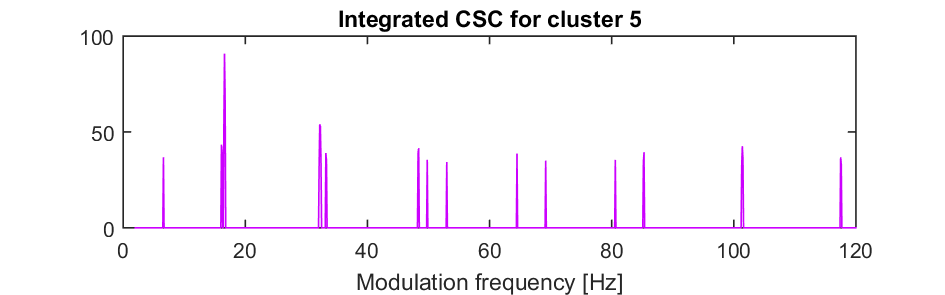
\includegraphics[width=\textwidth]{wykresy/212_cluster_sum_5.png}
\caption{The Integrated Spectral Coherence map of the cluster containing information about the damage on the first shaft.}
\label{fig:intSC5}
\end{center}
\end{figure}

The presented results show that the SC map can be automatically clustered and information about several different faults can be extracted and separated.

 It is worth mentioning that the usage of the appropriate number of clusters is crucial. Each of the signal components should be assigned to a different cluster. Indeed, in the analyzed signal two clusters are automatically created containing the components related to two different local damages. 
\newpage
\section{Conclusions}
In this paper the bi-frequency cyclostationary map has been considered. The well known Cyclic Spectral Coherence has been computed in order to extract information about local damage on gears from a vibration signal. CSC has been proven as a powerful tool for condition monitoring of the rotating machinery. However, it is often analyzed only visually and in case of signals with many different cyclic components its interpretation can be challenging. Therefore in this paper an automatic method has been proposed applying a clustering approach on the CSC map. The EM method, applied on the SC, has been used in order to cluster the different subsignals. The proposed methodology was tested and evaluated on real vibration data capture on a belt conveyor operating in a harsh environment in an underground copper mine. The analyzed belt conveyor had two local gear faults (mounted on the first and the second shaft). Based on the results, it is shown that the proposed method is able to automatically assign the information about separate local damages to different clusters, facilitating the diagnostic procedure. 

% \begin{figure}[t]
% \begin{center}
% 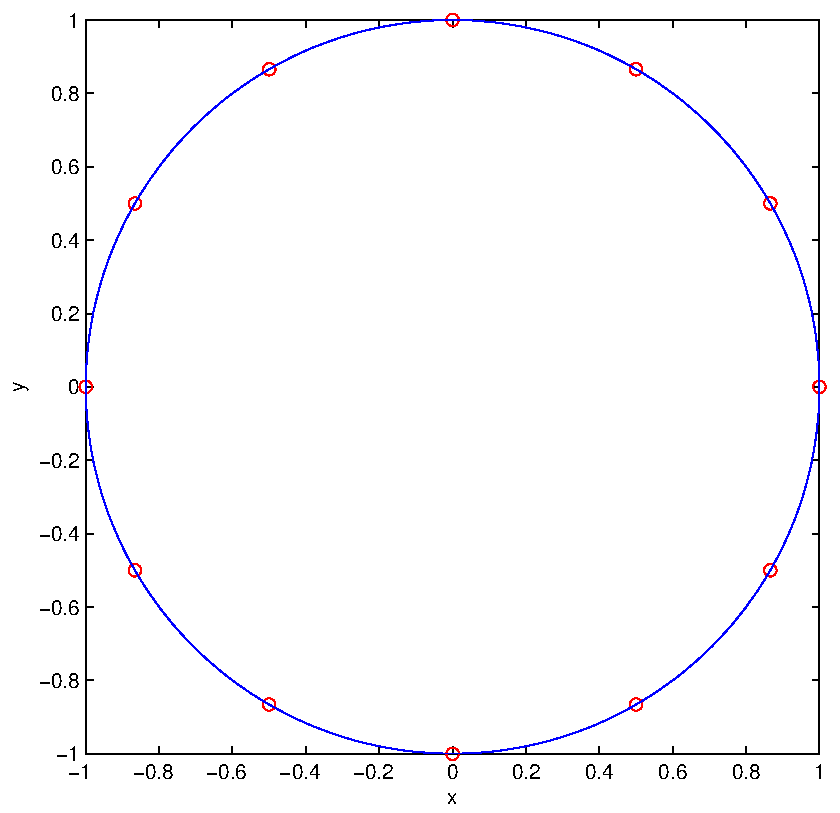
\includegraphics[width=80mm]{circle_rgb}
% \caption{$x = \cos \phi$ and $y = \sin \phi$ \label{f:circle}}
% \end{center}
% \end{figure}

% \begin{table}[ht]
% \centering
% \begin{tabular}{c|cc}
% $\phi$   & $x = \cos \phi$ & $y = \sin \phi$ \\
% \hline
% $0$      &    $1$          &    $0$          \\
% $\pi/6$  &  $\sqrt{3}/2$   &    $1/2$        \\
% $\pi/3$  &    $1/2$        &  $\sqrt{3}/2$   \\
% $\pi/2$  &    $0$          &    $1$
% \end{tabular}
% \caption{Quarter of a circle \label{t:circle}}
% \end{table}




\section*{Acknowledgements}
The work of R.Zimroz and J.Wodecki was supported by the statutory grant.

\bibliographystyle{ISMA}
\bibliography{mybib}

% \begin{thebibliography}{1}

% \bibitem{heylen}
%   W. Heylen, S. Lammens, P. Sas,
%   \textit{Modal Analysis Theory and Testing},
%   Katholieke Universiteit Leuven, Departement Werktuigkunde, Leuven (1997).

% \bibitem{sas}
%   P. Sas, C. Bao, F. Augusztinovicz, W. Desmet,
%   \textit{Active control of sound transmission through a double panel partition},
%   Journal of Sound and Vibration, Vol. 180, No. 4, Academic Press (1995), pp. 609-625.

% \bibitem{boonen}
%   R. Boonen, P. Sas,
%   \textit{Modified Smith Compensation for Feedback Active Noise Control in Ducts},
%   in \mbox{R. Boone}, editor,
%   \textit{Proceedings of The 2001 International Congress and Exhibition
%       on Noise Control Engineering, The Hague, The Netherlands, 2001 August 27-30},
%   The Hague (2001), pp. 619-624.
% \end{thebibliography}




\end{document}
